\section{Prediction and cluster test results}\label{sec:testing}
To validated that the cluster gives us an improvement when working on big data, a list of tests will be explored. The first initial tests that will be performed, seen in \Cref{sec:initialtest}, will be run to find the settings the cluster should run with. In \Cref{sec:clustertest}, the tests run on the cluster and the results will be presented.

\subsection{Initial testing}\label{sec:initialtest}
In this section several tests will be performed which does not require the cluster. These tests will be run to find the settings the cluster should be run with when the final cluster tests will be performed.

\subsubsection{Best machine learning technique}
First the best machine learning technique needs to be identified. In this test six different methods are included, these are: naive bayes, hidden naive bayes, logistic regression, neural network, support vector machines(SVM) and adaboost. All the different methods are tested with multiple parameter settings to find the configuration that yields the best result. The feature representation used for this test is binary representation, presented in \Cref{sec:representationoffeatures}, and 35000 matches are used. The data will be split, using $\frac{2}{3}$ for training and $\frac{1}{3}$ for testing. 

The best accuracy of all the machine learning technique can be seen in \Cref{fig:besttech}. As seen, SVM and Neural networks has the worst accuracy, even after testing different parameter configurations. Naive bayes, adaboost and Hidden naive bayes all have comparable results around 56.5\%, but logistic regression has the best accuracy almost hitting 57\%, which will be the technique mainly used throughout these tests.  

% \begin{figure}[!htb]
%   \begin{tikzpicture}
%     \begin{axis}[
%       x tick label style={/pgf/number format/1000 sep=},
%       ylabel=Accuracy,
%       xlabel=Parameter configuration,
%       enlargelimits=0.05,
%       legend style={at={(0.5,1.1)},
%         anchor=north,legend columns=-1},
%       ybar interval=0.7,
%       width=.75\textwidth,
%       ymin=56, ymax=57,
%       ]
%       \addplot[fill=red] coordinates {(13,56.5462) 
%         (12,56.6218) 
%         (11,56.8403) 
%         (10,56.8319) 
%         (9,56.916) 
%         (8,56.8487) 
%         (7,56.8655) 
%         (6,56.6471) 
%         (5,56.6471) 
%         (4,56.605) 
%         (3,56.605) 
%         (2,56.5882) 
%         (1,56.5798) 
%         (0,2)
%       };
%       \addplot[fill=blue] coordinates {(13,56.4454) 
%         (12,56.4454) 
%         (11,56.4454) 
%         (10,56.4454) 
%         (9,56.4454) 
%         (8,56.4454) 
%         (7,56.4454) 
%         (6,56.4454) 
%         (5,56.4454) 
%         (4,56.4454) 
%         (3,56.4454) 
%         (2,56.4454) 
%         (1,56.4454) 
%         (0,56.4454)
%       };
%       \addplot[fill=green] coordinates {(13,56.6807) 
%         (12,56.6807) 
%         (11,56.6807) 
%         (10,56.6807) 
%         (9,56.6807) 
%         (8,56.6807) 
%         (7,56.6807) 
%         (6,56.6807) 
%         (5,56.6807) 
%         (4,56.6807) 
%         (3,56.6807) 
%         (2,56.6807) 
%         (1,56.6807) 
%         (0,56.6807)
%       };
%       \addplot[fill=orange] coordinates {(13,0) 
%         (12,0) 
%         (11,0) 
%         (10,0) 
%         (9,0) 
%         (8,49.87) 
%         (7,56.2269) 
%         (6,56.479) 
%         (5,56.1261) 
%         (4,55.5126) 
%         (3,54.7899) 
%         (2,54.5378) 
%         (1,53.7983) 
%         (0,2)
%       };
%       \addplot[fill=black] coordinates {(13,0) 
%         (12,0) 
%         (11,0) 
%         (10,0) 
%         (9,0) 
%         (8,0) 
%         (7,0) 
%         (6,0) 
%         (5,50.1) 
%         (4,55.6555) 
%         (3,52.7311) 
%         (2,55.5126) 
%         (1,50.2101) 
%         (0,0)
%       };
%       \addplot[fill=purple] coordinates {(13,0)
%         (12,0)
%         (11,0)
%         (10,0)
%         (9,0)
%         (8,0)
%         (7,0)
%         (6,0)
%         (5,0)
%         (4,55.3193)
%         (3,55.63)
%         (2,51.521)
%         (1,55.5714)
%         (0,0)
%       };
%       \legend{Logistic Regression,Naive Bayes,Hidden Naive Bayes,Adaboost,Neural Network,SVM}
%     \end{axis}
%   \end{tikzpicture}
%   \caption{Test of best machine learning technique}\label{fig:besttech}
% \end{figure}

\begin{figure}[!htb]
  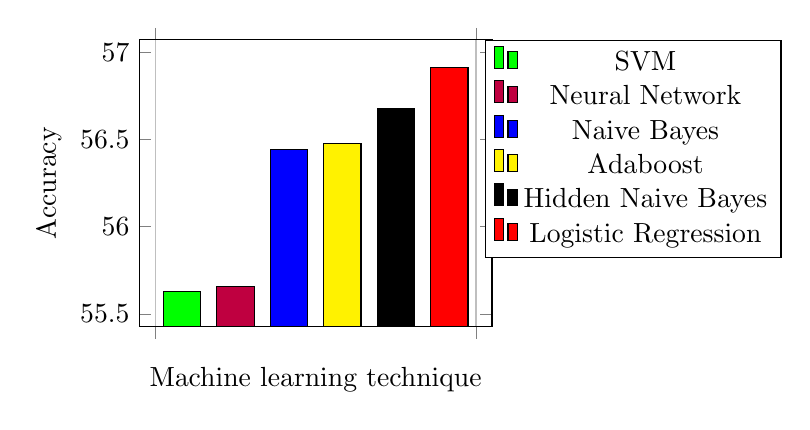
\begin{tikzpicture}
    \begin{axis}[
      %x tick label style={/pgf/number format/1000 sep=},
      xticklabel=\empty,
      ylabel=Accuracy,
      xlabel=Machine learning technique,
      enlargelimits=0.05,
      legend style={at={(1.4,1.0)},
        anchor=north,legend columns=1},
      ybar interval=0.7,
      width=.50\textwidth,
      ymin=55.5, ymax=57,
      reverse legend,
      ]
      \addplot[fill=red] coordinates {(1,56.916) 
        (0,2)
      };
      \addplot[fill=black] coordinates {(1,56.6807) 
        (0,56.6807)
      };
      \addplot[fill=yellow] coordinates {(1,56.479) 
        (0,2)
      };
      \addplot[fill=blue] coordinates {(1,56.4454) 
        (0,56.4454)
      };
      \addplot[fill=purple] coordinates {(1,55.6555) 
        (0,0)
      };
      \addplot[fill=green] coordinates {(1,55.63)
        (0,0)
      };
      \legend{Logistic Regression,Hidden Naive Bayes,Adaboost,Naive Bayes,Neural Network,SVM}
    \end{axis} 
  \end{tikzpicture}
  \caption{Test of best machine learning technique}\label{fig:besttech}
\end{figure}



\subsubsection{Implementation comparison}
To test if Apache Sparks PySpark implementation of logistic regression is implemented properly, it is compared to the equivalent implementations in Weka and R. The data consists of 5000 matches where Weka uses a sparse presentation, while R uses a dense and PySpark the raw file with JSON elements. As seen in \Cref{tab:impl_results}, the implementations are close to equal, the minor differences could be caused by differences in the parameter settings. However these results confirm that all implementations are acceptable and further testing can be performed in any of the environments.

\begin{table}[!htb]
  \centering
  \begin{tabular}{|l|c|}
    \hline
    Implementation  & Accuracy  \\
    \hline
    Weka & 55\%  \\
    R & 55\%\\
    PySpark & 53\%\\ 
    \hline
  \end{tabular}
  \caption{Implementation comparison results}
  \label{tab:impl_results}
\end{table}

\subsubsection{Feature representation test}
Features can be presented in many different ways and this test is constructed to finding the best way to that. The representations that will be tested are the methods presented in \Cref{sec:representationoffeatures}. The test was done on an increasing number of matches with all the different methods to check how they hold up with much data. As the result, shown in \Cref{fig:feat-rep}, indicates, method 1 and 4 are very close, but binary being slightly above ternary majority of the time, which is the reason for us choosing binary.

\begin{figure}[!htb]
  \centering
  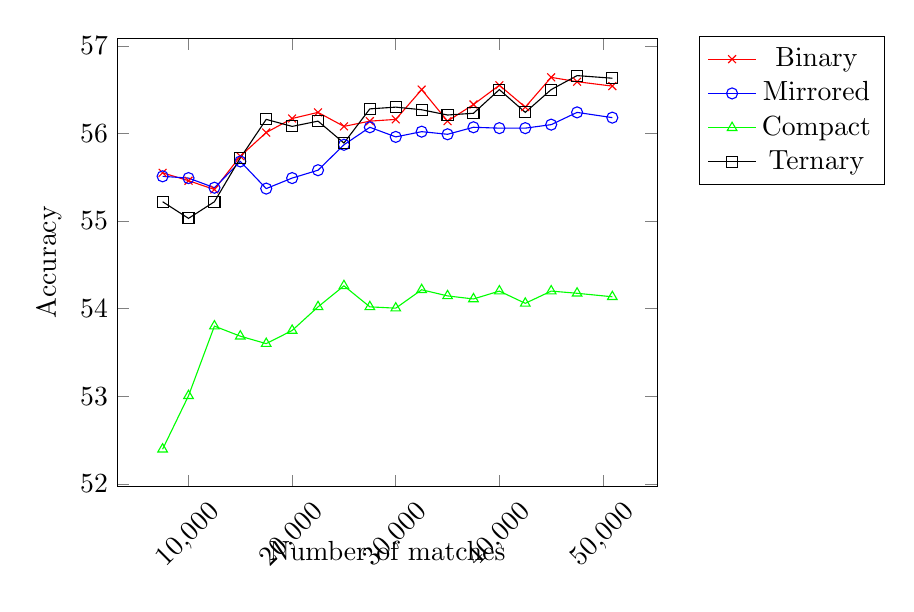
\begin{tikzpicture}[] 
    \begin{axis}[
      xlabel=Number of matches, 
      ylabel=Accuracy,
      xtick={10000,20000,30000,40000,50000},
      xticklabel style={rotate=45,anchor=near xticklabel},
      scaled x ticks=false,
      x label style={at={(axis description cs:0.5,-0.1)},anchor=north},
      legend style={at={(1.25,1.005)},
        anchor=north,legend columns=1},] 
      \addplot[color=red,mark=x] coordinates { 
        (7500, 55.55)
        (10000, 55.46)
        (12500, 55.36)
        (15000, 55.74)
        (17500, 56.01)
        (20000, 56.17)
        (22500, 56.24)
        (25000, 56.08)
        (27500, 56.14)
        (30000, 56.16)
        (32500, 56.50)
        (35000, 56.14)
        (37500, 56.33)
        (40000, 56.55)
        (42500, 56.30)
        (45000, 56.64)
        (47500, 56.59)
        (50901, 56.54)
      };
      \addplot[color=blue,mark=o] coordinates { 
        (7500, 55.51)  
        (10000, 55.49)
        (12500, 55.38)
        (15000, 55.68)
        (17500, 55.37)
        (20000, 55.49)
        (22500, 55.58)
        (25000, 55.87)
        (27500, 56.07)
        (30000, 55.96)
        (32500, 56.02)
        (35000, 55.99)
        (37500, 56.07)
        (40000, 56.06)
        (42500, 56.06)
        (45000, 56.10)
        (47500, 56.24)
        (50901, 56.18)
      };
      \addplot[color=green,mark=triangle] coordinates { 
        (7500, 52.395)  
        (10000, 53.005)
        (12500, 53.80)
        (15000, 53.685)
        (17500, 53.60)
        (20000, 53.75)
        (22500, 54.02)
        (25000, 54.26)
        (27500, 54.02)
        (30000, 54.005)
        (32500, 54.215)
        (35000, 54.145)
        (37500, 54.11)
        (40000, 54.20)
        (42500, 54.06)
        (45000, 54.20)
        (47500, 54.175)
        (50901, 54.135)
      };
      \addplot[color=black,mark=square] coordinates {
        (7500, 55.22)  
        (10000, 55.03)
        (12500, 55.22)
        (15000, 55.72)
        (17500, 56.16)
        (20000, 56.08)
        (22500, 56.14)
        (25000, 55.89)
        (27500, 56.28)
        (30000, 56.30)
        (32500, 56.27)
        (35000, 56.21)
        (37500, 56.23)        
        (40000, 56.50)
        (42500, 56.24)
        (45000, 56.50)
        (47500, 56.66)
        (50901, 56.63)
      };
      \legend{Binary, Mirrored, Compact, Ternary}
    \end{axis} 
  \end{tikzpicture}
  \caption{Test for representation of features}\label{fig:feat-rep}
\end{figure}

\subsubsection{Feature tests}\label{sec:feattest}
Some features might be more expressive than others, and finding the set of features that will yield the best result is imperative. The test on the cluster is performed with logistic regression using stochastic gradient descent and L2 regularization with a ridge value of 0.01. 
For each feature test 1348428 games is used for training and 577552 games are used for evaluation. 
The feature sets tested are:
\begin{enumerate}
\item blue team, purple team 
\item blue pairs, purple pairs
\item blue team, purple team, blue pairs, purple pairs
\item blue team, purple team, blue pairs, purple pairs, counter pairs
\item blue team, purple team, blue pairs, purple pairs, counter pairs, champion ranks
\item all pre-match features 
\end{enumerate}

For each set of features the total possibilities of features is given, as well as the amount of features extracted from a single game. Along with the numbers is given a reasoning for testing the features.  
\\\\
\textbf{Blue team, purple team} \\
As mentioned in \Cref{sec:onlinevideogames} each team picks 5 champions, from a pool of 124 champions, this results in a total of 248 features, of which 10 is picked. The feature representation to test the importance of the individual champions. \\\\
\textbf{Blue pairs, purple pairs} \\
As mentioned in  \Cref{sec:choosingfeatures} there might be some synergy between combinations of champions. The total number pairs for each team is calculated as $n \times (n-1)/2$. The total amount of features is calculated as:  
\begin{itemize}
\item $124 \times (124-1)/2 + 124 \times (124-1)/2 = 15252$
\end{itemize}
From the possible features $20$ is represented for each match. \\\\
\textbf{Blue team, purple team, blue pairs, purple pairs} \\
This feature test is added to test how well the extension from team to pairs works with the individual players. The total features are: 
\begin{itemize}
\item $248 + 15252 = 15500$
\end{itemize}
The total features pick for each game is 30.\\\\
\textbf{Blue team, purple team, blue pairs, purple pairs, counter pairs}\\
The counter pairs is calculated as $n^2$, the purpose of this feature is to capture champions which have special skills which counters the skills on another champion. The total features for counter pairs is: 
\begin{itemize}
\item $15500+124\times124 = 30876$
\end{itemize}
From this pool of features 55 is represented in each match.\\\\
\textbf{Blue team, purple team, blue pairs, purple pairs, cross team pairs, champion ranks}\\
For each player their best achieved rank in the previous season is known there are 8 possible ranks. The total features for this test is: 
\begin{itemize}
\item $30876 + 124\times8 = 31868$
\end{itemize}
From this pool of features 65 is represented in each match. \\\\
\textbf{All pre-match features}\\
All pre-match features is a combination of, blue team, purple team, blue pairs, purple pairs, cross team pairs, champion ranks, champions lanes, best team rank, champion queue type, champion runes, champion masteries and champion spell pair.  

Champion lanes describe which lane a given champion is played on e.g. a champion might perform better if played in the middle lane instead of the top lane. Best team rank is a measure of how skilled the two teams are. Champion queue type combines the champion picked by a player with the game mode being played. Champion runes combines the champion picked with the runes of the player who picked the champion (runes are used to boot certain skills of a champion, e.g. give a champion higher starting health). Champion masteries, masteries have the same purpose as runes. Champion spell pair is a combination of the champion picked and the summoner spells picked by the player. The total possible features of this test is 189.183. The amount of features represented in each game varies a lot e.g. some players might have 30 different runes resulting in 30 features for that player another player might not have any runes resulting in only 1 feature.
\begin{figure}[!htb]
  \centering
  % Graph for feature tests. 
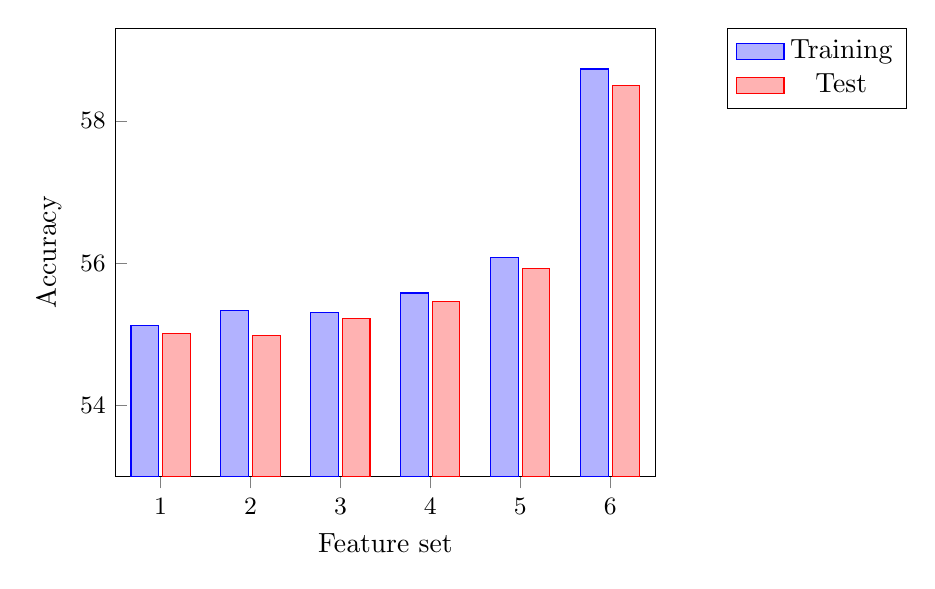
\begin{tikzpicture}
\begin{axis}[
    ybar,
    ylabel = Accuracy,
    xlabel = Feature set,
    tick label style={font=\small},
    tickpos=left,
    xticklabels={1, 2, 3, 4, 5, 6}, 
    xtick={1,2,3,4,5, 6},
    ymin=53,
    legend entries={Training,Test},
    legend style={at={(1.3,1.0)},
        anchor=north,legend columns=1
    },
    legend image code/.code={%
      \draw[#1] (0cm,-0.1cm) rectangle (0.6cm,0.1cm);
    }   
    ]   
    \addplot +[bar shift=-.2cm] coordinates {(1,55.12) (2,55.34) (3,55.31)  (4,55.58)     (5,56.08)  (6, 58.73)};

    \addplot  +[bar shift=.2cm]coordinates {(1,55.01) (2,54.98) (3,55.22) (4,  55.46) (5,55.92) (6, 58.50)};

\end{axis}
\end{tikzpicture}
   \caption{Accuracy of features}\label{fig:cluster-feat}
\end{figure}

The feature evaluation results from \Cref{fig:cluster-feat} shows two interesting results, by looking at each individual test case we see the we have almost no over fitting. The largest difference is blue pairs, purple pairs with a difference of $3.610^{-3}$ percentage points. The results shows some tendency between the complexity of the model and the performance of the classifier. Higher complexity in general yields a better classifier. The best result was achieved using all pre-match features.
\begin{figure}[!htb]
  \centering
  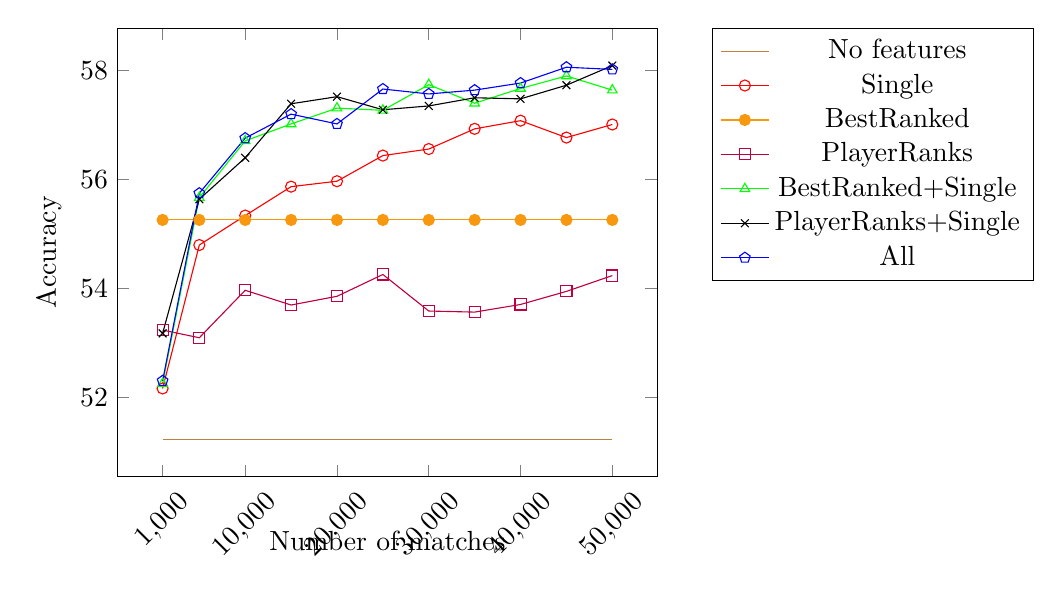
\begin{tikzpicture}[] 
    \begin{axis}[
      xlabel=Number of matches, 
      ylabel=Accuracy,
      xtick={1000,10000,20000,30000,40000,50000},
      xticklabel style={rotate=45,anchor=near xticklabel},
      scaled x ticks=false,
      x label style={at={(axis description cs:0.5,-0.1)},anchor=north},
      legend style={at={(1.4,1.001)},
        anchor=north,legend columns=1},] 
      \addplot[color=brown] coordinates { 
        (1000,51.24)
        (5000,51.24)
        (10000,51.24)
        (15000,51.24)
        (20000,51.24)
        (25000,51.24)
        (30000,51.24)
        (35000,51.24)
        (40000,51.24)
        (45000,51.24)
        (50000,51.24)
      };
      \addplot[color=red,mark=o] coordinates { 
        (1000,52.17)
        (5000,54.8)
        (10000,55.34)
        (15000,55.87)
        (20000,55.97)
        (25000,56.44)
        (30000,56.56)
        (35000,56.93)
        (40000,57.08)
        (45000,56.77)
        (50000,57.01)
      };
      \addplot[color=YellowOrange,mark=*] coordinates { 
        (1000,55.26)
        (5000,55.26)
        (10000,55.26)
        (15000,55.26)
        (20000,55.26)
        (25000,55.26)
        (30000,55.26)
        (35000,55.26)
        (40000,55.26)
        (45000,55.26)
        (50000,55.26)
      };
      \addplot[color=purple,mark=square] coordinates { 
        (1000,53.24)
        (5000,53.1)
        (10000,53.97)
        (15000,53.7)
        (20000,53.86)
        (25000,54.26)
        (30000,53.59)
        (35000,53.57)
        (40000,53.71)
        (45000,53.95)
        (50000,54.24)
      };
      \addplot[color=green,mark=triangle] coordinates { 
        (1000,52.26)
        (5000,55.67)
        (10000,56.71)
        (15000,57.02)
        (20000,57.31)
        (25000,57.27)
        (30000,57.74)
        (35000,57.4)
        (40000,57.67)
        (45000,57.9)
        (50000,57.64)
      };
      \addplot[color=black,mark=x] coordinates { 
        (1000,53.18)
        (5000,55.64)
        (10000,56.4)
        (15000,57.39)
        (20000,57.52)
        (25000,57.28)
        (30000,57.35)
        (35000,57.5)
        (40000,57.48)
        (45000,57.73)
        (50000,58.09)
      };
      \addplot[color=blue,mark=pentagon] coordinates { 
        (1000,52.31)
        (5000,55.75)
        (10000,56.76)
        (15000,57.2)
        (20000,57.02)
        (25000,57.66)
        (30000,57.57)
        (35000,57.64)
        (40000,57.77)
        (45000,58.06)
        (50000,58.02)
      };
      \legend{No features,Single,BestRanked,PlayerRanks,BestRanked+Single,PlayerRanks+Single,All}
    \end{axis} 
  \end{tikzpicture}
  \caption{Accuracy of features}\label{fig:best-feat}
\end{figure}

\subsection{Cluster tests}\label{sec:clustertest}
In this section the tests that requires the cluster. This is due to the size of the tests, and the expected time frame.
\subsubsection{Big data on the cluster}
One of the key points of this project was working on big data, to test the improvement of the classifier as the training size increases. A experiments using only a percentage of the 1348428 games used in \Cref{sec:feattest} is used to for training and 577552 games are used for evaluation. The features uses is all pre-match features. The classifier used in this test is logistic regression with stochastic gradient descent with L2 regularization and a ridge value of 0.01. The size of the training set used are as follows: 
\begin{enumerate}
\item 84529 matches
\item 168431 matches 
\item 337146 matches 
\item 674438 matches
\item 1348428 matches 
\end{enumerate}
% Graph for big data testing. 
\begin{figure}[!htb]
  \centering
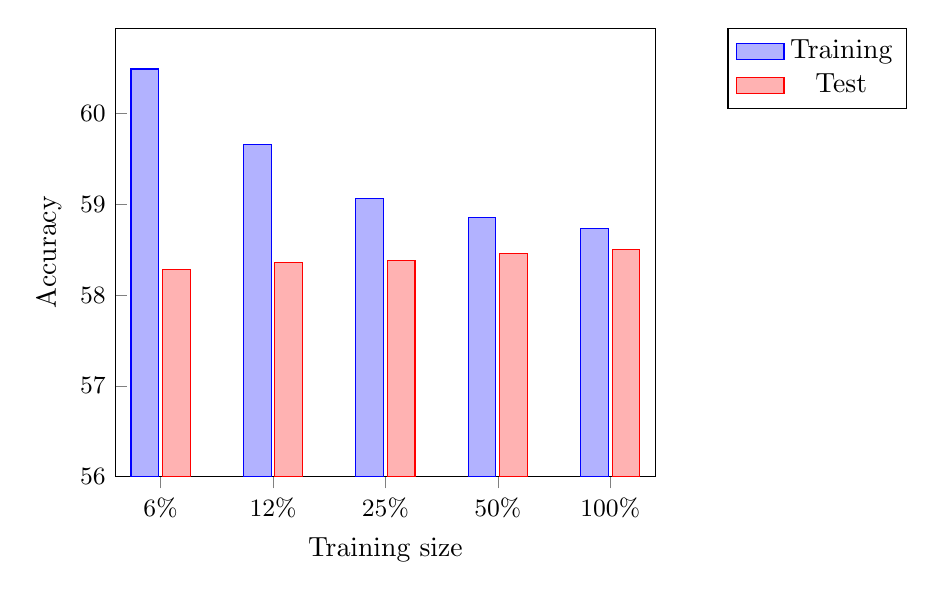
\begin{tikzpicture}
\begin{axis}[
    ybar,
    ylabel = Accuracy,
    xlabel = Training size,
    tick label style={font=\small},
    tickpos=left,
    xticklabels={6\%, 12\%, 25\%, 50\%, 100\%}, 
    xtick={1,2,3,4,5, 6},
    ymin=56,
    legend entries={Training,Test},
    legend style={at={(1.3,1.0)},
        anchor=north,legend columns=1
    },
    legend image code/.code={%
      \draw[#1] (0cm,-0.1cm) rectangle (0.6cm,0.1cm);
    }   
    ]   
    \addplot +[bar shift=-.2cm] coordinates {(1,60.49) (2,59.66) (3,59.06)  (4,58.85)     (5,58.73)  };

    \addplot  +[bar shift=.2cm]coordinates {(1,58.28) (2,58.36) (3,58.38) (4,  58.46) (5,58.50) };

\end{axis}
\end{tikzpicture}
  \caption{Test for representation of features}\label{fig:clusterbigdata}
\end{figure}
The results from \Cref{fig:clusterbigdata} shows that as more data is used to train the model the prediction accuracy on the test set increases the total change from 84529 matches to 134828 matches is $3.86\times10^{-1}\%$

The results also shows the as the size of the training data increases overfitting decreases. The difference in accuracy between the training set and test set moves from $3.79\%$ for $84529$ matches to $3.79\times10^{-1} \%$ for $1348428$ matches. The result shows that the model do not improve a lot as the amount of data increases. The test shows that as the amount of data used for training increases overfitting decreases.      
\subsubsection{Big data improvements}
To test if big data gives an improvement when predicting the outcome of a match, the same features and method where used on an increasing sized data starting from 1000 matches. After the model was made, it was tested on the training data, as a $\frac{2}{3}$-split and finally cross-validation. And as seen on \Cref{fig:bigdata} there will be more information once more tests has been run!

\begin{figure}[!htb]
  \centering
  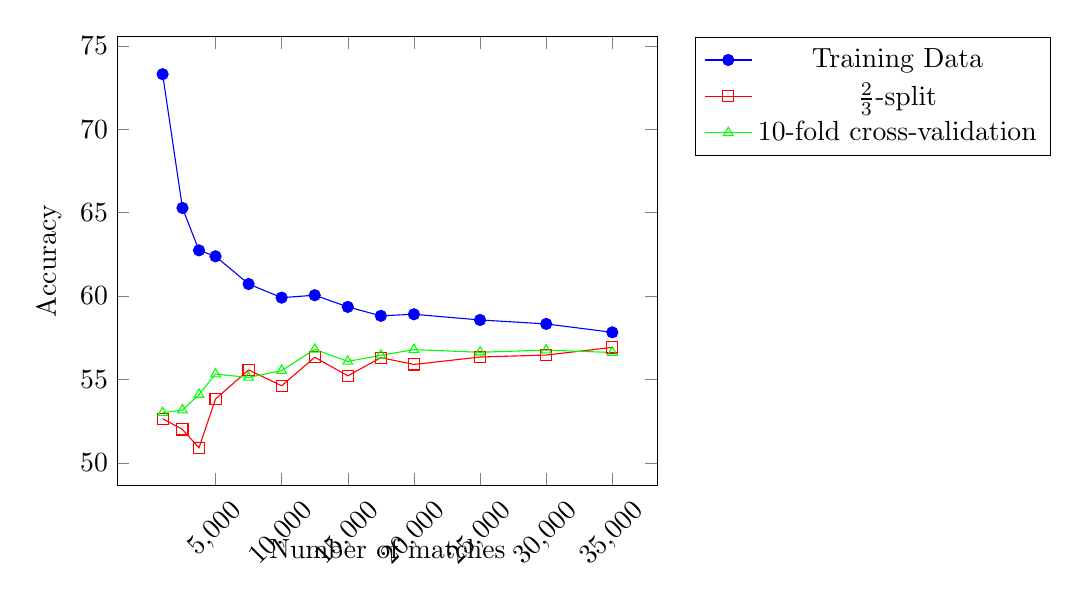
\begin{tikzpicture}[] 
    \begin{axis}[
      xlabel=Number of matches, 
      ylabel=Accuracy,
      xtick={5000,10000,15000,20000,25000,30000,35000},
      xticklabel style={rotate=45,anchor=near xticklabel},
      scaled x ticks=false,
      x label style={at={(axis description cs:0.5,-0.1)},anchor=north},
      legend style={at={(1.4,1.0)},
        anchor=north,legend columns=1},] 
      \addplot[color=blue,mark=*] coordinates {
        (1000, 73.3)   	
        (2500,65.28)  	
        (3750,62.7367)	
        (5000,62.38)
        (7500,60.72)
        (10000,59.9)
        (12500,60.048)
        (15000,59.3467)
        (17500,58.8114)
        (20000,58.905)
        (25000,58.564)
        (30000,58.3267)
        (35000,57.8229)
      };
      \addplot[color=red,mark=square] coordinates {
        (1000,52.6471)
        (2500,52)
        (3750,50.902)
        (5000,53.8235)
        (7500,55.5686)
        (10000,54.6176)
        (12500,56.3294)
        (15000,55.2157)
        (17500,56.3025)
        (20000,55.8971)
        (25000,56.3412)
        (30000,56.4608)
        (35000,56.916)
      };
      \addplot[color=green,mark=triangle] coordinates {
        (1000,53)
        (2500,53.16)
        (3750,54.0944)
        (5000,55.32)
        (7500,55.12)
        (10000,55.53)
        (12500,56.8)
        (15000,56.08)
        (17500,56.4457)
        (20000,56.785)
        (25000,56.628)
        (30000,56.7567)
        (35000,56.6143)
      };
      \legend{Training Data, $\frac{2}{3}$-split, 10-fold cross-validation}
    \end{axis} 
  \end{tikzpicture}
  \caption{Test for representation of features}\label{fig:bigdata}
\end{figure}

\subsubsection{Speed up}
This test is constructed to show that an increasing number of nodes increases the computation speed. As seen in \Cref{sec:clustersetup}, the cluster consists of 4 nodes, this means the test will be run with the master and either 1, 2 or 3 nodes. The data for this test be the same to make the results comparable.

\begin{table}[!htb]
  \centering
  \begin{tabular}{|c|c|}
    \hline
    Number of nodes & Time taken\\
    \hline
    1 & ? \\
    2 & ? \\
    3 & ? \\
    \hline
  \end{tabular}
  \caption{Speed up test results}\label{tab:speedup}
\end{table}

\subsubsection{Prediction with team ranks}
Previous seasons rank for each player is registered in the match data. This test is constructed to test whether this rank alone is a useful feature when predicting a winning team.
\subsubsection{Prediction with all features}
All the features created from the data is used for this test. 
\subsubsection{Prediction with all features except lane}
This test is almost identical to the test seen above, except the lane feature is excluded. This test is performed to learn if the lane each hero choses to defend influences the outcome of the match and if this is actually useful when predicting outcome of future matches.
\subsubsection{Prediction using support vector machine}
The above tests will for this test be performed using support vector machine to see how it compares to logistic regression. 
\subsubsection{Prediction with best features}
The test for prediction with best features will use the features that were determined as the best in \Cref{sec:feattest}. This is done to see how well the prediction can be made at all. This should, should we play the game, give us the opportunity to pick champions that counter those of the opponents team, thus increasing our chances of winning.
\subsubsection{Sample size}
Text.


%%% Local Variables:
%%% mode: latex
%%% TeX-master: "../main"
%%% End:
